\documentclass[11pt]{article}

\def\chapitre{8}
\def\pagetitle{Séries entières.}

\input{setup.tex}

\begin{document}

\input{title.tex}

\thispagestyle{fancy}

\begin{defi}{}{}
    Une série entière est une série de fonctions particulières, de la forme $\sum u_n$ avec $\forall n\in \N, ~ u_n : x \mapsto a_nx^n$.\\
    Les sommes partielles d'une série entière sont donc des fonctions polynomiales.
    \begin{equation*}
        \forall n \in \N, ~ S_n(x) = \sum_{k=0}^\infty a_kx^k.
    \end{equation*}
    Si $(a_n)_n\in\K^\N$, avec $(a_n)_n$ nulle àpdcr, alors $S$ est une fonction polynomiale.\\
    \smallwarning En général, la somme n'est pas une fonction polynomiale.
\end{defi}

\section{Étude de séries entières.}

\subsection{Rayon de convergence.}

\begin{defi}{}{}
    Soient $(a_n)_n \in \K^n$ et $E=\{r \geq 0, ~ (a_n r^n)_n ~ \nt{bornée}\}$.\\
    Le rayon de convergence (RCV) de la série entière $\sum a_nx^n$ est défini par : $R=\sup E$.
    \tcblower
    On va montrer que $E$ est de la forme $[0,R[$ ou $[0,R]$.\\
    $\hookrightarrow$ On remarque que $0\in E$ car $(a_n0^n)_n = (a_0, 0, ...)$.\\
    $\hookrightarrow$ De plus, $r \in E$ et $0 \leq r' < r \ra r' \in E$ car $\exists M \geq 0, ~ \forall n \in \N, ~ |a_nr'^n|\leq |a_nr^n|\leq M$.\\
    Ainsi, $\forall (r,r') \in E^2, ~ r' < r \ra [r',r]\subset E$, c'est une partie convexe de $\R$, donc c'est un intervalle.\\
    Donc $E$ est un intervalle de $\R_+$, contenant $0$, il est de la forme $[0,R[$ ou $[0,R]$.
\end{defi}

\begin{nota}{}{}
    Par abus de notation, on confondra dans tout le chapitre l'écriture $\sum_{n\geq0}a_nx^n$ et $\sum_{n\geq0}(x\mapsto a_nx^n)$.
\end{nota}

\vspace*{-0.8cm}

\begin{ex}{}{}
    \begin{itemize}
        \item Si $\forall n \in \N, ~ a_n = 1$, alors : $(a_nr^n)$ bornée ssi $(r^n)$ bornée ssi $r\in[0,1]$, donc $E=[0,1]$.
        \item Soit $\a>0$, si $\forall n \in \N, ~ a_n = \frac{1}{\a^n}$, alors : $(a_nr^n)$ bornée ssi $\left(\left(\frac{r}{\a}\right)^n\right)$ bornée ssi $r\in [0,\a]$, donc $E=[0,\a]$.
        \item Si $\forall n \in \N, ~ a_n = n$, alors : $(a_nr^n)$ bornée ssi $(nr^n)$ bornée ssi $r\in[0,1[$ (d'Alembert) donc $E=[0,1[$.
        \item Si $\forall n \in \N, ~ a_n = n!$, alors : $(a_nr^n)$ bornée ssi $(n!r^n)$ bornée ssi $r=0$, donc $E=\{0\}$. ($R=0$)
        \item Si $\forall n \in \N, ~ a_n = \frac{1}{n!}$, alors : $(a_nr^n)$ bornée ssi $\left(\frac{r^n}{n!}\right)$ bornée ssi $r\in[0,+\infty[$, donc $E=[0,+\infty[$. ($R=+\infty$)
    \end{itemize}
    \bf{Remarque.} Soit $(a_n)_n\in\K^\N$, alors $\sum a_n z^n$ et $\sum |a_n|x^n$ ont même rayon de convergence.\\
    En effet, pour $z\in\C$, $(a_nz^n)$ bornée ssi $\exists M > 0, |a_nz^n|=|a_n||z|^n\leq M$ ssi $(|a_n||z|^n)$ bornée. 
\end{ex}

\vspace*{-0.8cm}

\begin{thm}{de comparaison.}{}
    Soient $(a_n)_n, (b_n)_n \in (\R_+)^\N$ de rayons de convergence $R_a$ et $R_b$.
    \begin{enumerate}
        \item Si $a_n \leq b_n$ àpdcr, alors $R_b \leq R_a$.
        \item Si $a_n \sim_\infty b_n$, alors $R_a = R_b$.
    \end{enumerate}
    \tcblower
    \boxed{1.} On a $a_n \leq b_n$ àpdcr $\ra E_b \subset E_a \ra \sup E_b \leq \sup E_a\ra R_b \leq R_a$ car $(b_nr^n)$ bornée $\ra$ $(a_nr^n)$ bornée.\\
    \boxed{2.} On a $a_n = b_n(1+\e_n)$ avec $\e_n \to 0$, donc $\exists N\in\N, ~ \forall n \geq N, ~ \frac{1}{2}\leq 1 + \e_n \leq \frac{3}{2}$ puis $\frac{1}{2}b_n \leq a_n \leq \frac{3}{2}b_n$.\\
    On remarque que $\sum a_n x^n$ et $\sum \l a_nx^n$ ont même rayon pour tout $\l\in\R^*$, puis par $1$, $R_a \leq R_b$ et $R_b \leq R_a$.
\end{thm}

\vspace*{-0.8cm}

\begin{ex}{}{}
    \begin{itemize}
    \item Pour $n\in\N$, on pose $a_n=e^{in\theta}\frac{n^2+3n+2}{4n+1}$. Alors $|a_n|=\frac{n^2+3n+2}{4n+1}\sim\frac{n}{4}$ puis $R_a=1$.
    \item Pour $n\in\N$, soit $(a_n)\in\R^\N$ telle que $1 \leq a_n \leq n$. Alors $R_a = 1$.
    \end{itemize}
\end{ex}

\vspace*{-0.8cm}

\subsection{Convergence.}

\begin{defi}{}{}
    Soit $\sum a_nz^n$ une série entière de rayon de convergence $R$. On notera $D(0,R)$ le disque ouvert de convergence.
    \begin{itemize}
        \item Si $\K=\R$, alors $D(0,R)=]-R,R[$.
        \item Si $\K=\C$, alors $D(0,R)=\{z\in \C, ~ |z|<R\}$.
    \end{itemize}
\end{defi}

\vspace*{-0.8cm}

\begin{thm}{Lemme d'Abel. $\star$}{}
    Soient $(a_n)_n\in\K^\N$ et $z_0\in\C$ tel que $(a_nz_0^n)_n$ bornée.
    \begin{equation*}
        \forall z \in \C, ~ |z| < |z_0| \ra \sum_{n\geq0} a_nz^n ~ \CA
    \end{equation*}
    \tcblower
    Soit $z\in\C, ~ |z|<|z_0|$. On montre la convergence absolue de la série numérique.
    \begin{equation*}
        \forall n \in \N, ~ |a_nz^n| = |a_n||z|^n = |a_n||z_0|^n\left(\frac{|z|}{|z_0|}\right)^n
    \end{equation*}
    Par hypothèse, $\exists M > 0, ~ \forall n \in \N, ~ |a_nz_0^n| \leq M$ donc $|a_nz^n|\leq M\left( \frac{|z|}{|z_0|} \right)^n$ terme général de série convergente.\\
    Par TCSTG+, $\sum|a_nz^n|$ converge, donc la série converge absolument.
\end{thm}

\begin{thm}{Convergence.}{8}
    Soit $(a_n)_n \in \K^\N$. Notons $R$ le rayon de convergence de la série entière.
    \begin{enumerate}
        \item $\sum a_nz^n$ $\CA$ sur $D(0,R)$.
        \item $\sum a_nz^n$ diverge grossièrement pour $z \notin D(0,R)$ ($|z|>R$).
        \item $\sum a_nz^n$ $\CN$ puis $\CU$ sur tout $B'(0,r)$, avec $r<R$. 
        \item Il y a incertitude sur le bord du disque, pour $|z|=R$.
    \end{enumerate}
    \tcblower
    \boxed{1.} Soit $z\in D(0,R)$, i.e. $|z|<R$. Soit $|z_0|\in \C, ~ |z|<|z_0|<R$. Alors $|z_0|<R\ra|z_0|\in E \ra (a_nz_0^n)$ bornée.\\
    Donc, par lemme d'Abel, la série converge absolument.\\
    \boxed{2.} Soit $z\in\K$, $|z|>R$, on a $z\notin E$, donc $(a_nz^n)$ non bornée, donc $a_nz^n\not\to0$, donc diverge grossièrement.\\
    \boxed{3.} Soit $r\in[0,R[$. $\forall z \in B'(0,r), ~ \forall n \in \N, |a_nz^n|\leq|a_n|r^n$, $\|a_nz^n\|_{\infty}^{B'(0,r)}\leq|a_n|r^n$.\\
    Par TCSTG+, $\sum\|a_nz^n\|_\infty^{B'(0,r)}$ converge, donc convergence normale.
\end{thm}

\vspace*{-0.8cm}

\begin{ex}{}{}
    \begin{enumerate}
        \item $\forall n \in \N, ~ a_n = 1$, $\sum z^n$, $R=1$.
        \item $\forall n \in \N^*, ~ a_n = \frac{1}{n}$, $R=1$. Divergence en 1, convergence en $-1$.
        \item $\forall n \in \N^*, ~ a_n = \frac{1}{n^2}$, $R=1$, convergence en $1$ et $-1$.
    \end{enumerate}
\end{ex}

\vspace*{-0.8cm}

\begin{prop}{Remarques utiles pour le calcul du rayon.}{}
    Soit $(a_n)_n\in\K^\N$, et $R$ le rayon de convergence de $\sum a_nz^n$.
    \begin{enumerate}
        \item Si $\sum a_nz_0^n$ converge, alors $R\geq |z_0|$. ($z_0\in D(0,R)$ ou bord)
        \item Si $\sum a_nz_0^n$ diverge, alors $R\leq |z_0|$. ($z_0\notin D(0,R)$ ou bord)
        \item Si $(a_n)_n$ bornée, alors $R\geq1$ car $1\in E$.
        \item Si $\sum a_n$ diverge, alors $R\leq 1$ car $1\notin D(0,R)$.
    \end{enumerate}
\end{prop}

\vspace*{-0.8cm}

\begin{ex}{}{}
    Soit $a_n$ la $n^{\nt{ème}}$ décimale de $\pi$. Calculer le rayon de convergence de $\sum a_nx^n$.
    \tcblower
    Déjà, $\forall n \in \N, ~ a_n \in \lb0,9\rb$, donc $(a_n)$ bornée, donc $R\geq1$.\\
    De plus, $a_n\not\to0$, car sinon $(a_n)$ est nulle àpdcr, or $\pi$ est irrationnel... absurde.\\
    Donc $\sum a_n$ est grossièrement divergente, donc $R\leq 1$, donc $R=1$ par antisymétrie.
\end{ex}

\vspace*{-0.8cm}

\begin{ex}{}{}
    Soit une série entière $\sum a_nx^n$ de rayon de convergence $R$. Quel est le rayon de convergence de $\sum a_n R^nx^n$ ?
    \tcblower
    Notons $R'$ le RCV de $\sum a_nR^nx^n$. Si $R=0,$ alors $R'=+\infty$. Sinon, vérifions $R'=1$ :\\
    $\hookrightarrow$ Si $|x|<1$, alors $|Rx|<R$ puis $\sum a_n(Rx)^n$ converge.\\
    $\hookrightarrow$ Si $|x|>1$, alors $|Rx|>R$, puis $\sum a_n(Rx)^n = \sum a_nR^nx^n$ diverge.\\
    Donc $R'=1$.
\end{ex}

\pagebreak

\begin{thm}{Critère de d'Alembert spécifique aux séries entières.}{}
    Soit $(a_n)_n \in (R_+)^\N$ tel que $a_n\neq0$ àpdcr.
    \begin{center}
        \fbox{Si $\ds\frac{a_{n+1}}{a_n}\to l \in \ov{\R}$, alors $\ds R=\frac{1}{l}$.}
    \end{center}
    \vspace*{0.2cm}
    \bf{Remarque.} C'est le critère le plus facile à utiliser pour déterminer le RCV.
    \tcblower
    Posons $\forall n \in \N, ~ \forall x \in \R, ~ u_n(x)=a_nx^n$. On cherche $R$ RCV de la série entière $\sum u_n$.\\
    Soit $x\in\R^*$.
    \begin{equation*}\left|\frac{u_{n+1}(x)}{u_n(x)}\right|=\frac{a_{n+1}}{a_n}|x|\xrightarrow[n\to+\infty]{}l|x|.\end{equation*} 
    On utilise le critère de d'Alembert pour les séries numériques.\\
    $\hookrightarrow$ Si $l|x|<1$, alors $\sum|u_n(x)|$ converge, i.e. $\sum u_n(x)$ $\CA$ i.e. $|x|\leq R$.\\
    $\hookrightarrow$ Si $l|x|>1$, alors $\sum|u_n(x)|$ diverge, i.e. $|x|\geq R$.\n
    \bf{Remarque :} $\left[ \forall x, ~ |x|<a \ra |x|\leq b \right] \ra a \leq b$.\\
    $\hookrightarrow$ Si $|x|<\frac{1}{l}$, alors $|x|\leq R$, donc $\frac{1}{l}\leq R$.\\
    $\hookrightarrow$ Si $|x|>\frac{1}{l}$, alors $|x|\geq R$, donc $\frac{1}{l}\geq R$.\\
    Donc $R=\frac{1}{l}$.
\end{thm}

\vspace*{-0.8cm}

\begin{ex}{}{}
    Déterminer le rayon de convergence des séries suivantes :
    \begin{align*}
        &\bullet ~ \sum_{n\geq0} n^2x^n ~ : \quad \forall n \geq 1, ~ a_n = n^2, ~ \frac{a_{n+1}}{a_n}=\frac{(n+1)^2}{n^2}\to 1 \ra R=1.\\
        &\bullet ~ \sum_{n\geq0} \frac{\ln(n^2+3)}{\ln(2n^3+5)}x^n ~ : \quad \forall n \in \N, ~ a_n \sim \frac{2\cancel{\log n}}{3\cancel{\log n}}, ~ \frac{a_{n+1}}{a_n}\sim 1 \ra R=1.\\
        &\bullet ~ \sum_{n\geq0} \frac{n^2+1}{n!}z^n ~ : \quad \forall n \in \N, ~ \frac{a_{n+1}}{a_n}=\frac{(n+1)^2+1}{n^2+1}\cdot\frac{1}{n+1}\to 0 \ra R=+\infty.\\
        &\bullet ~ \sum_{n\geq0}(-1)^n\binom{2n}{n}x^n ~ : \quad \frac{|a_{n+1}|}{|a_n|}=\frac{(2n+2)!}{((n+1)!)^2}\cdot\frac{(n!)^2}{(2n)!}=\frac{(2n+1)(2n+2)}{(n+1)^2} \to 4 \ra R=\frac{1}{4}.
    \end{align*}
\end{ex}

\vspace*{-0.8cm}

\begin{defi}{Série lacunaire.}{}
    Une série entière $\sum a_nx^n$ est dite lacunaire ssi $a_n=0$ pour une infinité de $n$.\\
    Un polynôme est une série entière lacunaire.
\end{defi}

On ne peut pas appliquer le critère aux séries lacunaires, mais ici $\sum x^{3n}$ converge ssi $|x|<3$, donc $R=1$.

\pagebreak

\subsection{Propriétés de la somme.}

\begin{exercice}{Formule de Cauchy.}{}
    Notons $f(z)=\sum_{n=0}^\infty a_nz^n$ avec $(a_n)\in\K^\N$, et $R>0$. Montrer que :
    \begin{equation*}
        \forall r < R, ~ a_n = \frac{1}{2\pi r^n} \int_0^{2\pi} e^{-in\theta} f(re^{i\theta})\nt{d}\theta.
    \end{equation*}
    \tcblower
    On a :
    \begin{align*}
        \int_0^{2\pi}e^{-in\theta}f(re^{i\theta})\nt{d}\theta &= \int_0^{2\pi}e^{-in\theta}\sum_{k=0}^{+\infty}a_k r^ke^{ik\theta} \nt{d}\theta = \int_0^{2\pi}\sum_{k=0}^{+\infty}a_kr^ke^{i(k-n)\theta}\nt{d}\theta\\
        &\overset{(*)}{=}\sum_{k=0}^{+\infty}a_kr^k\int_0^{2\pi}e^{i(k-n)\theta}\nt{d}\theta=2\pi a_n r^n
    \end{align*}
    (*) On pose $u_k=a_kr^ke^{i(k-n)\theta}$, on vérifie que $\sum_{k\geq0}u_k$ $\CU$ sur $[0,2\pi]$.
    \begin{equation*}
        \forall \theta \in [0,2\pi], ~ \forall k \in \N, ~ |u_k(\theta)|=|a_k|r^k
    \end{equation*}
    Puis $\|u_k\|_\infty=|a_k|r^k$ terme général d'une série convergente. Enfin, $\CN$ implique $\CU$.
\end{exercice}

\vspace*{-0.8cm}

\begin{prop}{}{unicite}
    Soient $(a_n)_n,(b_n)_n\in\K^\N$. 
    \begin{equation*} \exists r > 0, ~ \forall x \in D(0,r), ~ \sum a_nx^
        n = \sum b_nx^n \ra \forall n \in \N, ~ a_n=b_n. \end{equation*}
    \tcblower
    On le démontre avec la formule de Cauchy (Hors-Programme).
    Soit $0<p<r$. Par la formule de Cauchy :
    \begin{equation*}
        \forall n \in \N, ~ a_n = \frac{1}{2\pi p^n}\int_0^{2\pi}e^{-in\theta}f(pe^{i\theta})\nt{d}\theta = \frac{1}{2\pi p^n}\int_0^{2\pi}e^{-in\theta}g(pe^{i\theta})\nt{d}\theta = b_n
    \end{equation*}
    En particulier, $\sum_{n=0}^{+\infty}a_nx^n=0$ sur un domaine non trivial $D(0,r)$ entraîne $\forall n \in \N, ~ a_n = 0$.
\end{prop}

\vspace*{-0.8cm}

\begin{ex}{}{}
    Soit $\sum a_nx^n$ une série entière de rayon de convergence $R>0$.
    \begin{equation*}
        \forall x \in ]-R, R[, ~ f(x) = \sum_{n=0}^\infty a_n x^n
    \end{equation*}
    Vérifions $f$ paire $\ra$ $\forall n \in \N, ~ a_{2n+1}=0$.
    \tcblower
    On a :
    \begin{equation*}
        \forall x \in ]-R,R[, ~ f(-x)=f(x), ~ \sum_{n=0}^{+\infty}(-1)^na_nx^n = \sum_{n=0}^{+\infty}a_nx^n.
    \end{equation*}
    Par le théorème précédent, $\forall n \in \N, ~ (-1)^na_n = a_n$, puis $a_{2n+1}=0$.
\end{ex}

\vspace*{-0.6cm}

\begin{prop}{Continuité des séries entières.}{}
    Soit $(a_n)_n \in \K^\N$, et $f(z)=\sum_0^\infty a_nz^n$ de rayon de convergence $R$.\\
    Alors $f$ est continue sur $D(0,R)$.
    \tcblower
    \boxed{\R} On pose $\forall n \in \N, ~ \forall x \in ]-R,R[, ~ u_n(x)=a_nx^n$. Par théorème :\\
    $\hookrightarrow$ $\forall n \in \N, ~ u_n$ est continue sur $]-R,R[$.\\
    $\hookrightarrow$ $\sum u_n$ $\CN$ donc $\CU$ sur tout segment de $]-R,R[$ (\ref{thm:8}).\\
    Donc $f$ est continue sur $]-R,R[$.\n
    \boxed{\C} On pose $\forall n \in \N, ~ \forall z \in D(0,R), ~ u_n(z)=a_nz^n$.\\
    On a $\forall n \in \N, ~ u_n$ est continue sur $D(0,R)$ et $\sum u_n$ $\CN$ donc $\CU$ sur $B'(0,R)$.\\
    Vérifions que $f$ est continue en $z_0\in D(0,R)$. Soit $r\in\R,  ~ |z_0| < r < R$.\\
    Par théorème de continuité des séries de fonctions sur $B(0,r)$, puis $z_0\in B(0,r)$, donc $f$ continue en $z_0$.
\end{prop}

\vspace*{-0.6cm}

\begin{lemme}{}{}
    Soit $(a_n)\in\K^\N$.
    \begin{enumerate}
        \item $\sum_{n\geq0}a_nz^n$ et $\sum_{n\geq0}na_nz^n$ ont même rayon de convergence.
        \item $\forall p \in \Z, ~ \sum_{n\geq0}a_nz^n$ et $\sum_{n\geq0}n^pa_nz^n$ ont même rayon de convergence.
    \end{enumerate}
    \bf{Le critère de d'Alembert ne fonctionne pas ici.}
    \tcblower
    \boxed{1.} Notons $R$ le rayon de convergence de $\sum a_nz^n$ et $R'$ le rayon de convergence de $\sum na_nz^n$.\\
    $\hookrightarrow$ $\forall n \geq 1, ~ |a_n|\leq n|a_n|$ et par comparaison, $R'\leq R$.\\
    $\hookrightarrow$ Soit $z\in\K$ tq $|z|<R$. Montrons que $\sum na_nz^n$ converge.\\
    Soit $r\in \R, ~ |z|<r<R$. $\forall n \in \N, ~ |na_nz^n|=|a_n|r^nn\left( \frac{|z|}{r} \right)^n$.\\
    Puisque $r<R$, $(a_nr^n)_n$ est bornée : $\exists M > 0, ~ \forall n \in \N, ~ |a_nr^n|\leq M$.\\
    Donc $\forall n \in \N, ~ |na_nz^n|\leq M n\left( \frac{|z|}{r} \right)^n$ terme général de série convergente.\\
    Par TCSTG+, $\sum|na_nz^n|$ converge, ie $\sum na_nz^n$ converge absolument.\\ 
    Puis $|z|\leq R'$ ($z$ dans $D(0,R)$ ou sur le bord). Par double inégalité, $R=R'$.\\
    \boxed{2.} Par récurrence sur $p$, $\forall p \in \N, ~ \sum n^pa_nz^n$ a même rayon que $\sum a_nz^n$.\\
    Puis d'après le 1, $\sum \frac{a_n}{n}z^n$ a même rayon de convergence que $\sum a_nz^n$, puis par récurrence pour $p\in \Z$.
\end{lemme}

\pagebreak

\begin{thm}{Dérivation de séries entières.}{}
    Soit $(a_n)_n\in\R^\N$. On pose $S(x)=\sum^{\infty}a_nx^n$ de rayon de convergence $R$.\\
    Alors $S$ est $\cursive{C}^\infty(]-R,R[)$. On peut dériver terme à terme et toutes les séries dérivées ont même rayon de convergence $R$.\\
    De plus, $\forall n \in \N, ~ a_n = \frac{S^{(n)(0)}}{n!}$. Si $R=+\infty$, même comportement qu'un polynôme.
    \tcblower
    Vérifions déjà que $S$ est $\cursive{C}^1(]-R,R[)$ et que $\forall x \in ]-R,R[, ~ S'(x)=\sum_{n=1}^\infty na_nx^{n-1}$.\\
    On pose $\forall n \in \N, ~ \forall x \in ]-R,R[, ~ u_n=a_nx^n$.\\
    On applique le théorème de dérivation des séries de fonctions :\\
    $\hookrightarrow$ $\forall n \in \N, ~ u_n$ est $\cursive{C}^1$ et $u'_n(x)=na_nx^{n-1}$.\\
    $\hookrightarrow$ $\sum u_n'$ $\CU$ sur $]-R,R[$ (*).\\
    Donc $S$ est $\cursive{C}^1$ et $\forall x \in ]-R,R[$, ~ $S'(x)=\sum_{n=0}^\infty u_n'(x)=\sum_{n=1}^\infty na_nax^{n-1}$.\\
    Vérifions $(*)$ :\\
    $\hookrightarrow$ $\sum u_n'(x) = \sum na_nx^{n-1}$.\\
    $\hookrightarrow$ $\sum u_n'$ $\CN$ donc $\CU$ sur tout segment de $]-R',R'[$ et $R=R'$ par lemme précédent.\\
    Vérifions que $S$ est $\cursive{C}^\infty$ sur $]-R,R[$ ie $S\in\cursive{C}^p$ pour tout $p$ dans $\N$. Soit $p\in\N^*$.\\
    $\hookrightarrow$ $\forall n \in \N, ~ u_n$ est $\cursive{C}^p$ sur $]-R,R[$.\\
    $\hookrightarrow$ $\forall k \in \lb0,p-1\rb$, $\sum u_n^{(k)}$ $\CS$ sur $]-,R,R[$.\\
    $\hookrightarrow$ $\sum u_n^{(p)}$ $\CN$ donc $\CU$ sur tout segment de $]-R,R[$.
    \begin{equation*}
        \forall n \in \N, ~ \forall x \in ]-R,R[,  ~ S^{(n)}(x)=\sum_{k=0}^\infty a_k(x^k)^{(n)}.
    \end{equation*}
    Pour $n>k$, $(x^k)^{(n)}=0$, sinon $(x^k)^{(n)}=\frac{k!}{(k-n)!}x^{k-n}$. Donc :
    \begin{equation*}
        \forall x \in ]-R,R[, ~ S^{(n)}(x)=\sum_{k=n}^\infty a_k\frac{k!}{(k-n)!}x^{k-n} + \sum_{k=n+1}^\infty a_k\frac{k!}{(k-n)!}x.
    \end{equation*}
    On évalue en 0: $S^{(n)}(0)=n!a_n$ donc $S(x)=\sum_{n=0}^\infty\frac{S^{(n)(0)}}{n!}x^n$.
\end{thm}

\begin{ex}{}{}
    Soit $P\neq0\in\R[X]$ de degré $N$. C'est une série entière. Par la formule précédente: $\forall x \in \R, ~ P(x)=\sum_0^\infty\frac{P^{(n)(0)}}{n!}x^n$.\\
    Or $P^{(n)}=0$, pour $n>N$ il reste $P(x)=\sum_{n=0}^N\frac{P^{(n)(0)}}{n!}x$.
\end{ex}

\begin{prop}{Primitivation d'une série entière.}{}
    Soit $(a_n)\in\K^\N$, $S(x)=a_nx^n$ de rayon de convergence $R$. Elle est bien définie sur $]-R,R[$.\\
    Alors $S$ est primitive terme à terme sur $]-R,R[$ avec conservation du rayon $R$.
    \tcblower
    Idée de preuve.\\
    On pose $T(x)=\sum_{n=0}^\infty a_n\frac{x^{n+1}}{n+1}=\sum_{n=1}^\infty\frac{a_{n-1}}{n}x^n$. rcv R'.\\
    D'après le théorème précédent, $T$ est $\cursive{C}^1$  invariance du rayon, et $\forall x \in ]-R',R'[, ~ T'(x)=S(x)$ donc $R=R'$.
\end{prop}

\begin{ex}{}{}
    \begin{equation*}
        \forall x \in ]-1,1[, ~ S(x)=\sum_{n=0}^\infty x^n \quad R=1 ~\et~ S(x)=\frac{1}{1-x}.
    \end{equation*}
    On sait que $S$ est $\cursive{C}^\infty$ sur $]-1,1[$. On peut dériver terme à terme avec conservation du rayon.
    \begin{equation*}
        \forall x \in ]-1,1[, ~ \sum_{n=0}^\infty x^n=\frac{1}{1-x}; \qquad \sum_{n=0}^\infty nx^{n} = \frac{x}{(1-x)^2}.
    \end{equation*}
    \begin{equation*}
        \forall x \in ]-1,1[, ~ \sum_{n=0}^\infty n^2x^{n-1}=\frac{x(x+1)}{(1-x)^3}.
    \end{equation*}
    On peut primitiver :
    \begin{equation*}
        \forall x \in ]-1,1[, ~ \sum_{n=0}^\infty\frac{x^{n+1}}{n+1}=-\ln(1-x)+\cancel{C}
    \end{equation*}
\end{ex}

\vspace*{-0.8cm}

\begin{ex}{}{}
    \begin{equation*}
        \sum_{n=0}^\infty \sh(n)x^n.
    \end{equation*}
    Rayon de convergence ?
    \tcblower
    On pose $a_n = \sh(n)=\frac{e^{n}-e^{-n}}{2}\sim \frac{e^n}{2}$, puis $\frac{e^{n+1}}{e^n}\to e$ donc $R=\frac{1}{e}$.\\
    Puis, $\forall x \in ]-\frac{1}{e},\frac{1}{e}[, ~ S(x)=\sum_{n=0}^\infty(\sh n)x^n=\frac{1}{2}\sum_{n=0}^\infty (ex)^n - \frac{1}{2}\sum_{n=0}^\infty\left( \frac{x}{e} \right)^n$.\\
    Alors $S(x)=\frac{1}{2}\frac{1}{1-ex}-\frac{1}{2}\frac{1}{1-e/x}$.
\end{ex}

\vspace*{-0.8cm}

\begin{ex}{}{}
    \begin{equation*}
        \forall z \in \C, ~ \sum_{n=0}^{\infty}(-2)^n\frac{z^n}{n!}=e^{-2z}.
    \end{equation*}
    Donc $R=+\infty$.
    \begin{equation*}
        \sum_{n=0}^\infty\frac{n+1}{n!}z^n=\sum_{n=1}^\infty\frac{z^n}{(n-1)!}+\sum_{n=0}^\infty\frac{z^n}{n!}=e^z(z+1).
    \end{equation*}
    \begin{equation*}
        \sum\frac{n^3+4n+1}{n!}z^n = e^z + 5ze^z + 3z^2e^z + z^3e^z
    \end{equation*}
    $n^3+4n+1=1+5n+3n(n+1)+5(n-1)(n-2)$ 
\end{ex}

\vspace*{-0.8cm}

\begin{ex}{}{}
    \begin{equation*}
        \sum_{n=0}^{\infty}\frac{z^{2n+1}}{(2n+1)!}
    \end{equation*}
    On sait que $\forall z \in \C, ~ \sum_{n\geq0} \frac{z^n}{n!}$ $\CA$ puis $\sum\frac{z^{2n+1}}{(2n+1)}$ $\CA$, donc $R=+\infty$.
    \begin{equation*}
        e^z - e^{-z} = \sum_{n=0}^\infty\frac{1-(-1)^n}{n!}z^n = 2\sum_{n=0}^\infty\frac{z^{2n+1}}{(2n+1)!}
    \end{equation*}
    \begin{equation*}
        \sh(z) + \frac{1}{i}\sh(iz) = \sum_{n=0}^\infty \frac{1 + (-1)^n}{(2n+1)!}z^{2n+1} = 2\sum_{n=0}^\infty\frac{z^{4n+1}}{(4n+1)!}.
    \end{equation*}
\end{ex}

\begin{thm}{Continuité aux bords, Abel radial.}{}
    Soit $\sum a_nx^n$ une série entière de rayon de convergence $R\in\R_+^*$. On note $S(x)=\sum a_nx^n$ bien définie sur $]-R,R[$. Si $S$ est définie en $R$, alors $S$ est continue en $R$.
    \tcblower
    \bf{Supposons $R=1$}.\\
    1er cas : $\sum a_n$ converge absolument, alors on pose $\forall n \in \N, ~ \forall x \in [0,1], ~ u_n(x)=a_nx^n$.
    \begin{equation*}
        \forall n \in \N, ~ \|u_n\|_\infty^{[0,1]}=\sup|u_n(x)|=|a_n|
    \end{equation*}
    $\sum u_n$ $\CN$ donc $\CU$ sur $[0,1]$, on applique le théorème de continuité des séries de fonctions :\\
    --- $\forall n \in \N, ~ u_n$ continue sur $[0,1]$.\\
    --- $\sum u_n$ $\CU$ sur $[0,1]$.\\
    Donc $S$ est continue sur $[0,1]$.\\
    2ème cas : $\sum a_n$ converge, mais pas absolument, alors on pose $\forall n \in \N ,~ \forall x \in [0,1], ~ u_n(x)=a_nx^n$.\\
    Posons $\forall n \in \N, ~ \forall x \in [0,1], ~ R_n(x)=\sum_{k=n+1}^\infty u_k(x)$.
    \begin{equation*}
        R_n(x) = \sum_{k=n+1}^\infty a_kx^k = \sum_{k=n+1}^\infty(A_{k-1} - A_k)x^k
    \end{equation*}
    \begin{equation*}
        \forall N \in \N, ~ N \geq n+1, ~ \sum_{k=n+1}^N(A_{k-1}-A_k)x^k=A_nx^{n+1}-A_Nx^N + \sum_{k=n+1}^{N-1}A_k(x^{k+1}-x^k)
    \end{equation*}
    Puis $\forall x \in [0,1], ~ |A_Nx^N|\leq A_N \xrightarrow[N\to+\infty]{} 0$, donc $A_nx^N\to 0$.
    \begin{equation*}
        \forall n \in \N, ~ \forall x \in [0,1], ~ R_n(x) = \sum_{k=n+1}^\infty A_k(x^{k+1}-x^k) + A_nx^{n+1}
    \end{equation*} 
    puis $\forall n \in \N, ~ \forall x \in [0,1], ~ |R_n(x)|\leq\sum_{k=n+1}^\infty|a_k|(x^k-x^{k+1})+|A_n||x^{n+1}|$.\\
    Soit $\e>0$, ~ $\exists N \in \N, ~ \forall n \geq N$, $|A_n|\leq\e$ puis $|R_n(x)|\leq \e x^{n+1} + \e \leq 2\e$.\\
    Donc $\|R_n\|_\infty \leq 2\e$. Donc $R_n\cu 0$ sur $[0,1]$, donc $S$ continue sur $[0,1]$.\n
    \bf{Supposons $R\in\R$}.\\
    On pose $\forall x \in [0,1[, ~ T(x)=S\left(Rx\right)$ :
    \begin{equation*}
        \forall x \in [0,1[, ~ T(x) = \sum_{n=0}^\infty(a_nR^n)x^n
    \end{equation*} 
    On a $T$ définie en 1 $\ra$ $T$ continue en 1 $\ra$ $S$ continue en $R$.\n
    \bf{Continuité en $-R$ si $S$ définie en $-R$.}\\
    On pose $T(x)=S(-x)$, les deux séries ont même rayon de convergence $R$.
    \begin{equation*}
        T(x)=\sum_{n=0}^\infty(-1)^na_nx^n
    \end{equation*}
    puis $T$ définie en $R$ ssi $S$ définie en $(-R)$ et $T$ définie en $R$ $\ra$ $T$ continue en $R$.
\end{thm}

\begin{ex}{}{}
    Existence et calcul de :
    \begin{equation*}
        \sum_{n\geq1}\frac{(-1)^{n+1}}{n}.
    \end{equation*}
    \tcblower
    L'existence vient du CSSA car décroissante vers 0. On pose $S$ la somme, et $S_n$ les sommes partielles.\\
    Pour calculer $S$, il faut connaître la limite de n'importe quelle suite extraite de $S_n$.
    \begin{equation*}
        S_{2n} = \sum_{k=1}^{2n}\frac{1}{k} - 2\sum_{k=1}^n\frac{1}{2k} = H_{2n} - H_n = \ln(2) + o(1) \to \ln(2).
    \end{equation*}
    On peut le voir aussi comme une série entière évaluée en une valeur de $x$.
    \begin{equation*}
        S(x) = \sum_{n=1}^{\infty}\frac{x^n}{n}, \quad \forall n \in \N, ~ a_n = \frac{1}{n}.
    \end{equation*}
    On a alors $R=1$, par exemple avec d'Alembert. Définie sur $[-1,1[$ par CSSA, donc continue en $-1$ par Abel.
    \begin{equation*}
        \sum_{n=1}^\infty\frac{(-1)^{n+1}}{n} = -\sum_{n=1}^\infty\frac{(-1)^n}{n} = -S(-1) = - \lim_{x\to-1}S(x)
    \end{equation*}
    Or $S$ est $\cursive{C}^\infty$ sur $]-1,1[$, et $S'(x)=\sum_{n=0}^\infty x^n = \frac{1}{1-x}$, donc $\forall x \in ]-1,1[, ~  S(x)=-\ln(1-x)+\l$.\\
    On évalue en $0$, $\l=0$. Donc $\forall x \in ]-1,1[$, ~ $S(x)=-\ln(1-x)$.\\
    Par continuité de $\ln$, $\lim_{x\to-1}S(x)=-\ln(2)$ puis par Abel Radial, $S(-1)=-\ln(2)$.
\end{ex}

\pagebreak

\begin{exercice}{}{}
    \begin{equation*}
        S(x)=\sum_{n=0}^\infty a_nx^n, \quad a_n = \begin{cases}a_0=a_1=1\\ \forall n \in \N^*, ~ a_{n+1}=a_n+\frac{2}{n+1}a_{n-1}\end{cases}.
    \end{equation*}
    Démontrer que $\forall n \in \N^*, ~ 1 \leq a_n \leq n^2$.\\
    Déterminer $R$ et calculer $S(x)$ pour $x\in]-R,R[$.
    \tcblower
    Par récurrence double, $\forall n \in \N^*, ~ \P_n$ : << $1\leq a_n\leq n^2$ >>.\\
    \bf{Initialisation.} $1\leq a_1 = 1 \leq 1^2$, et $1 \leq a_2 = 2 \leq 4$.\\
    \bf{Hérédité.} Soit $n\in\N^*$ tel que $\P_n$ et $\P_{n+1}$.\\
    $\hookrightarrow$ $a_{n+2} = a_{n+1} + \frac{2}{n+2}a_n \geq 1 + \frac{2}{n+2}\cdot 1 \geq 1$.\\
    $\hookrightarrow$ $a_{n+2}\leq (n+1)^2 + \frac{2n}{n+1} \leq (n+2)^2$.\\
    Donc $\forall n \in \N^*, ~ \P_n$.\n
    \bf{Déterminons $R$.}\\
    On note $\forall n \in \N, ~ b_n=1$ et $c_n = n^2$. Alors $b_n \leq a_n \leq c_n$.\\
    Avec ddes notations évidents : $R_c \leq R_a \leq R_b$ (théorème de comparaison) puis $R_c=R_b=1$ par d'Alembert.\\
    Donc $R_a=1$ par encadrement.\n
    \bf{Calcul de $S(x)$ pour $x\in]-1,1[$.}\\
    On a $S$ de classe $\cursive{C}^\infty$ sur $]-1,1[$. On peut dériver terme-à-terme avec conservation du rayon :
    \begin{equation*}
        \forall x \in ]-1,1[, ~ S'(x) = \sum_{n=0}^{\infty}na_nx^{n-1}=\sum_{n=0}^{\infty}(n+1)a_{n+1}x^n.
    \end{equation*}
    Or $\forall n \geq 1, ~ (n+1)a_{n+1} = (n+1)a_n + 2a_{n-1}$, donc $(n+1)a_nx^n=na_nx^n+a_nx^n+(2a_{n-1}x^{n-1})x$.
    \begin{equation*}
        \sum_{n=1}^\infty(n+1)a_nx^n = \sum_{n=1}^\infty na_nx^n + \sum_{n=1}^\infty a_nx^n + 2x\sum_{n=1}^\infty a_{n-1}x^{n-1}.
    \end{equation*}
    Donc $S'(x)-a_1 = xS'(x) + S(x) - a_0 + 2xS(x)$ donc $S'(x) = \frac{2x+1}{1-x}S(x)$.
    \begin{equation*}
        \frac{2X+1}{1-X} = \frac{-2(1-X)+3}{1-X} = -2 + \frac{3}{1-X}, \quad \nt{décomposition en éléments simples}.
    \end{equation*}
    et $\int\frac{2x+1}{1-x}\dx=-2x-3\ln|1-x|$, une primitive sur $]1,1[$.\\
    Donc $S$ solution de l'EDL1 ssi $\exists \l \in \R, ~ \forall x \in ]-1,1[, ~ y(x)= \l e^{-2x-3\ln(1-x)}=\l\frac{e^{-2x}}{(1-x)^3}$.\\
    On évalue en 0:  $S(0)=1=\l$, donc $S(x)=\frac{e^{-2x}}{(1-x)^3}$ pour tout $x\in]-1,1[$.
\end{exercice}

\vspace*{-0.3cm}

\section{Développement en série entière.}

\subsection{Généralités.}

\begin{defi}{}{}
    Soit $f:A\subset \K \to \K$, où $A\in\cursive{V}(0)$ on dit que $f$ est développable en série entière en $0$ ssi $f$ est égale à la somme d'une série sur un domaine non trivial $D(0,r)$ avec $r>0$.\\
    C'est-à-dire $\exists (a_n)_n \in \K^\N, ~ \exists r > 0, \forall x \in ]-r,r[ ~ f(x)=\sum^\infty a_nx^n$.
\end{defi}

\vspace*{-0.3cm}

\begin{ex}{}{}
    \begin{equation*}
        \forall z \in \C\setminus\{1\}, ~ f(z) = \frac{1}{1-z}
    \end{equation*}
    est développable en série entière en 0, et $f(z)=\sum^\infty z^n$ pour tout $z\in D(0,1)$.\\
    Donc $f$ est égale à la somme d'une série entière sur un domaine non trivial.
\end{ex}

\vspace*{-0.3cm}

\begin{prop}{}{}
    Le développement en série entière, s'il existe, est unique (théorème \ref{prop:unicite}).
\end{prop}

\vspace*{-0.3cm}

\begin{prop}{}{}
    Si $f$ et $g$ sont développables en séries entières en $0$, alors $f+g$ et $fg$ aussi.
    \tcblower
    Supposons $f$ et $g$ développables en séries entières en $0$.\\
    $\hookrightarrow$ $\exists (a_n)\in\K^\N, ~ \exists r>0, ~ \forall x \in D(0,r), ~ f(x)=\sum_{n=0}^\infty a_nx^n$.\\
    $\hookrightarrow$ $\exists (b_n)\in\K^\N, ~ \exists r'>0, ~ \forall x \in D(0,r'), ~ g(x)=\sum_{n=0}^\infty b_nx^n$.\\
    Posons $r''=\max(r,r')$, alors $\forall x \in D(0,r''), ~ f(x)=\sum_{n=0}^\infty a_nx^n$ et $g(x)=\sum_{n=0}^\infty b_nx^n$.
    \begin{equation*}
        \forall x \in D(0,r''), ~ (f+g)(x) = f(x) + g(x) = \sum_{n=0}^\infty(a_n+b_n)x^n.
    \end{equation*}
    Donc $f+g$ est somme de séries entières sur un domaine non trivial, donc $f+g$ est développable en série entière.\\
    On a $\sum a_nx^n$ et $\sum b_nx^n$ $\CA$ sur $D(0,r'')$, donc la série produit de Cauchy $\sum c_nx^n$ $\CA$ sur $D(0,r'')$ et :
    \begin{equation*}
        \sum_{n=0}^\infty c_nx^n = \left( \sum_{n=0}^\infty a_nx^n \right)\left( \sum_{n=0}^\infty b_nx^n \right)
    \end{equation*}
    Donc $\forall x \in D(0,r''), ~ (fg)(x)=f(x)g(x)=\sum_{n=0}^\infty c_nx^n$, développable en série entière.
\end{prop}

\begin{prop}{}{}
    Soit $f$ développable en série entière en 0, $\exists r>0, ...$\\
    On sait que $f$ est $\cursive{C}^\infty$ sur $D(0,r)$, donc on peut dériver terme à terme avec conservation du rayon, donc toutes les dérivées de $f$ admettent un développement en série entière en 0, de même pour les primitives.
\end{prop}

\pagebreak

\begin{prop}{}{}
    Soit $f:V\in \cursive{V}(0) \to \K$ DSE en 0 et telle que $f(0)\neq0$. Alors $\frac{1}{f}$ est DSE en 0.
    \tcblower
    Par hypothèse :
    \begin{equation*}
        \exists r > 0, ~ \forall z \in D(0,r), \quad f(z) = \sum_{n=0}^\infty a_nz^n
    \end{equation*}
    La fonction $f$ est alors continue sur $D(0,r)$ et en particulier en zéro.\\
    Or $f(0)\neq0$ donc $f$ est non nulle au voisinage de 0, donc $\frac{1}{f}$ est définie sur un voisinage de 0.\\
    \bf{Analyse.} Supposons que $1/f$ admette un DSE en 0 :
    \begin{equation*}
        \exists r' > 0, ~ \forall z \in D(0,r'), \quad \frac{1}{f(z)}=\sum_{n=0}^\infty b_nz^n.
    \end{equation*}
    On pose $r''=\min(r,r')$. Alors par absolue convergence des DSE:
    \begin{align*}
        \forall z \in D(0,r''), ~ f(z)\cdot\frac{1}{f(z)}&=\left( \sum_{n=0}^\infty a_nz^n \right)\left( \sum_{n=0}^\infty b_nz^n \right)\\
        &=\sum_{n=0}^\infty\sum_{k=0}^n a_kz^kb_{n-k}z^{n-k} =\sum_{n=0}^\infty\left( \sum_{k=0}^n a_kb_{n-k}\right)z^n.
    \end{align*}
    Cela vaut aussi 1, donc par unicité du DSE en 0, \\
    Par récurrence forte, la suite $(b_n)_n$ est définie de manière unique.\\
    \bf{Synthèse.} On définit $(b_n)_n$ par récurrence forte. On pose $g(z)=\sum_{n=0}^\infty b_nz^n$.\\
    Ensuite, $f(z)g(z)=1$ donc $\frac{1}{f(z)}=g(z)=\sum b_n z^n$ sur un domaine non trivial.
\end{prop}

\begin{ex}{}{}
    Soit $(a_n)_n\in\R^\N$.
    \begin{equation*}
        \sum_{n\geq0}a_nx^n \quad\nt{a un RDC } R>0 \iff \exists q > 0, ~ \forall n \in \N, ~ |a_n|\leq q^n.
    \end{equation*}
\end{ex}

\begin{prop}{}{}
    Soit $f:V\in\cursive{V}(0)\to \R$.
    \begin{equation*}
        f \nt{ est DSE en 0} \ra f ~ \cursive{C}^\infty ~ \nt{ en 0}.
    \end{equation*}
    \tcblower
    Par hypothèse :
    \begin{equation*}
        \exists r > 0, ~ \forall x \in ]-r,r[, ~ f(x)=\sum_{n=0}^\infty a_nx^n.
    \end{equation*}
    On sait alors que $f$ est $\cursive{C}^\infty$ sur $]-r,r[$, donc $f$ est $\cursive{C}^\infty$ en 0.
\end{prop}

\begin{defi}{Série de Taylor.}{}
    Soit $f:V\in\cursive{V}(0)\to\R$ et $\cursive{C}^\infty$ en zéro. On définit sa série de Taylor :
    \begin{equation*}
        S_f(x) = \sum_{k=0}^{\infty}\frac{f^{(k)}(0)}{k!}x^k
    \end{equation*}
    \tcblower
    Si $f$ est DSE en 0, alors $\exists r > 0, ~ \forall x \in ]-r,r[, ~ f(x)=\sum a_nx^n$.\\
    On sait alors que $f$ est $\cursive{C}^\infty$ en 0 et que $\forall n \in\N, ~ a_n = \frac{f^{(n)}(0)}{n!}$ donc $f(x)=S_f(x)$ sur un domaine non trivial.\\
    Pour savoir si $f$ est égale à sa série de Taylor sur un domaine non trivial, on étudie la suite $(S_n)_n$, on cherche à vérifier si $S_n\cs f$ sur un domaine non trivial.\\
    On aura ensuite par unicité de la limite simple $f=S_f$ sur un domaine non trivial.\\
    Or $S_n \cs f$ sur $I$ $\iff$ $|f_n-S_n|\cs 0$ sur $I$ et on peut calculer $f(x)=S_n(x)$ par la formule de Taylor avec reste intégral :
    \begin{equation*}
        \forall n \in \N, ~ f(x) = \sum_{k=0}^n\frac{f^{(k)}(0)}{k!}x^k + \int_0^x \frac{(x-t)^n}{n!}f^{(n+1)}(t)\dt
    \end{equation*}
\end{defi}

\begin{app}{}{}
    Montrer que
    \begin{equation*}
        \forall x \in \R, ~ e^x = \sum_{n=0}^\infty\frac{x^n}{n!}. 
    \end{equation*}
    On sait que $e^x$ est $\cursive{C}^\infty$ en zéro et que $\forall n \in \N, ~ e^{(n)}(0)=1$.
    \begin{equation*}
        \forall n \in \N, ~ S_n(x)=\sum_{n=0}^\infty\frac{1}{n!}x^n
    \end{equation*}
    Notons $R$ le RCV de $\sum_{n\geq0}\frac{x^n}{x!}$, alors $R=+\infty$.\\
    Vérifions que $\forall x \in \R, ~ e^x = S_n(x)$. D'après la formule de Taylor :
    \begin{align*}
       \left| e^x - \sum_{k=0}^n\frac{x^k}{n!} \right| &= \left|\int_0^x\frac{(x-t)^n}{n!}e^{t}\dt\right| \leq e^x\int_0^x\frac{(x-t)^n}{n!}\dt \quad \nt{si } x\geq0\\
       &\leq e^x\left[ -\frac{(x-t)^{n+1}}{(n+1)!} \right]_0^x \leq e^x\frac{x^{n+1}}{(n+1)!}
    \end{align*} 
    Même majoration si $x\leq 0$ en inversant le signe. Finalement :
    \begin{equation*}
        \forall x \in \R, ~ \forall n \in \N, ~ \left|e^x-\sum_{k=0}^n\frac{x^k}{k!}\right|\leq e^{|x|}\frac{|x|^{n+1}}{(n+1)!}\to 0
    \end{equation*}
\end{app}

\subsection{Développements usuels.}

\begin{prop}{}{}
    Pour tout $z\in\C$, on a
    \begin{equation*}
        e^z = \sum_{n=0}^\infty\frac{z^n}{n!}
    \end{equation*}
    \begin{equation*}
        \ch(z) = \sum_{n=0}^\infty\frac{z^{2n}}{(2n)!}; \qquad \sh(z) = \sum_{n=0}^\infty\frac{z^{2n+1}}{(2n+1)!}
    \end{equation*}
    \begin{equation*}
        \cos(z) = \sum_{n=0}^\infty (-1)^n\frac{z^{2n}}{(2n)!}; \qquad \sin(z)=\sum_{n=0}^\infty(-1)^n\frac{z^{2n+1}}{(2n+1)!}
    \end{equation*}
\end{prop}

\vspace*{-0.8cm}

\begin{prop}{}{}
    Pour tout $z\in\C$ tel que $|z|<1$, on a
    \begin{equation*}
        \frac{1}{1-z} = \sum_{n=0}^\infty z^n; \qquad \frac{1}{1-z^2} = \sum_{n=0}^\infty z^{2n}
    \end{equation*}
    \begin{equation*}
        \frac{1}{1+z}= \sum_{n=0}^\infty(-1)^nz^n; \qquad \frac{1}{1+z^2} = \sum_{n=0}^\infty (-1)^nz^{2n}
    \end{equation*}
    On primitive terme-à-terme (avec conservation du rayon), pour $x\in]-1,1[$ :
    \begin{equation*}
        \ln(1-x) = -\sum_{n=1}^\infty \frac{x^{n}}{n}; \qquad \ln(1+x) = \sum_{n=1}^\infty (-1)^{n+1}\frac{x^n}{n}.
    \end{equation*}
    \begin{equation*}
        \arctan(x)=\sum_{n=0}^\infty(-1)^n\frac{x^{2n+1}}{2n+1}.
    \end{equation*}
\end{prop}

\vspace*{-0.8cm}

\begin{prop}{}{}
    Soit $\a\in\R$.
    \begin{equation*}
        \forall x \in ]-1,1[, ~ (1+x)^\a = 1 + \sum_{n=1}^\infty\frac{\a(\a-1)...(\a-(n-1))}{n!}x^n = \sum_{n=0}^\infty\binom{\a}{n}x^n.
    \end{equation*}
    \tcblower
    Si $\a\in\N$, c'est le binôme de Newton. Sinon, on pose $f:x\mapsto (1+x)^\a$.
    \begin{equation*}
        \forall x \in ]-1,1[, ~ (1+x)f'(x)=\a f(x) \quad \et \quad f(0)=1.
    \end{equation*}
    Par unicité des solutions d'un problème de Cauchy en EDL1, $f$ est l'unique solution.\\
    On va chercher une solution $y$ du problème développable en 0.\\
    Posons $\forall x \in ]-1,1[, ~ y(x)=\sum_{n=0}^\infty a_nx^n$, avec $R$ son rayon de convergence.\\
    On sait que $y$ est $\cursive{C}^1$ sur $]-R,R[$ donc $y'(x)=\sum_{n=0}^\infty(n+1)a_{n+1}x^n$. Ainsi :
    \begin{equation*}
        (1+x)g'(x)-\a g(x) = \sum_{n=0}^\infty((n+1)a_{n+1} + na_n - \a a_n)x^n
    \end{equation*}
    Par unicité du DSE en 0, $\forall n \in \N, ~ (n+1)a_{n+1}+na_n = \a a_n$ donc :
    \begin{equation*}
        \forall n \in \N, ~ a_{n+1} = \frac{\a-n}{n+1}a_n = \frac{\a(\a-1)...(\a-(n+1))}{n!}a_0 \et a_0=1.
    \end{equation*}
    On a trouvé une solution $y$ du problème, développable en 0, $y(0)=1$, donc par unicité $\forall x \in ]-1,1[, ~ f(x)=y(x)$.
\end{prop}

\begin{prop}{}{}
    Soit $x\in\R$.
    \begin{equation*}
        \arcsin(x) = \sum_{n=0}^\infty\frac{1}{4^n}\binom{2n}{n}\frac{x^{2n+1}}{2n+1}; \qquad \arccos(x)=\frac{\pi}{2} - \sum_{n=0}^\infty\frac{1}{4^n}\binom{2n}{n}\frac{x^{2n+1}}{2n+1}
    \end{equation*}
    \tcblower
    On a :
    \begin{equation*}
        (1-x)^{-\frac{1}{2}} = 1+\sum_{n=1}^\infty\frac{1}{4^n}\binom{2n}{n}x^n
    \end{equation*}
    Donc :
    \begin{equation*}
        \frac{1}{\sqrt{1-x^2}} = 1+\sum_{n=1}^\infty\frac{1}{4^n}\binom{2n}{n}x^{2n}.
    \end{equation*}
    On primitive terme-à-terme avec conservation du rayon.
    \begin{equation*}
        \arcsin(x) = x + \sum_{n=1}^\infty\frac{1}{4^n}\binom{2n}{n}\frac{x^{2n+1}}{2n+1} + \cancel{C}
    \end{equation*}
    Enfin, $\arccos(x)=\frac{\pi}{2}-\arcsin(x)$.
\end{prop}

\vspace*{-0.8cm}

\begin{prop}{}{}
    Soit $x\in\R$.
    \begin{equation*}
        \argsh(x) = \sum_{n=0}^\infty\frac{(-1)^n}{4^n}\binom{2n}{n}\frac{x^{2n+1}}{2n+1}
    \end{equation*}
    La fonction $\argch$ n'étant pas définie en 0, elle n'admet pas de DSE en 0.
    \tcblower
    Pour $x\in\R$,
    \begin{equation*}
        \argsh'(x) = \frac{1}{\sqrt{1+x^2}}; \qquad \argch'(x) = \frac{1}{\sqrt{x^2-1}}.
    \end{equation*}
\end{prop}

\vspace*{-0.8cm}

\subsection{Calculs de développements en série entière.}

Pas de compositions, on évite les quotients et les produits. On fait des sommes, des primitivations, des dérivations.

\begin{ex}{}{}
    On pose $f:x\mapsto e^{-\frac{1}{x^2}}$. Peut-on la développer en série entière.
    \tcblower
    Par récurrence sur $n\in\N$, $\forall x \in \R^*, ~ f^{(n)}(x)=P_n(\frac{1}{x})e^{-\frac{1}{x^2}}$ avec $P_n\in\R[X]$.\\
    \bf{Initialisation.} $P_0=1\in\R[X]$.\\
    \bf{Hérédité.} Pour $n\in\N$, on suppose la propriété au rang $n$.
    \begin{equation*}
        f^{(n+1)}(x)=\left( -\frac{1}{x^2}P_n'\left(\frac{1}{x}\right) \right)e^{-\frac{1}{x^2}} + \frac{2}{x^3}P_n\left( \frac{1}{x} \right)e^{-\frac{1}{x^2}}=\left( \frac{2}{x^3}P_n\left( \frac{1}{x} \right) - \frac{1}{x^2}P_n'\left( \frac{1}{x} \right) \right)e^{-\frac{1}{x^2}}.
    \end{equation*}
    On pose $P_{n+1}=2X^3P_n - X^2P_n' \in \R[X]$, donc $\forall n \in \N$, la propriété est vraie.\\
    Alors $f^{(n)}(x)\xrightarrow[x\to0]{}0$, et $f$ est $\cursive{C}^\infty$ en 0, avec $\forall n \in \N, ~ f^{(n)}(0)=0$.\\
    La série de Taylor associée à $f$ est donc nulle, or $f$ n'y est égale sur aucun voisinage de $0$ car $x\neq0\ra f(x)\neq0$, elle n'est pas DSE.
\end{ex}

\begin{ex}{}{}
    Donner les développements en série entière en zéro de $f$ :
    \begin{enumerate}
        \item $f(x)=\sin(x)\cos(x)$.
        \item $f(x)=\frac{\sin(4x)}{\sin(x)}$ et $f(0)=4$.
        \item $f(x)=\frac{1}{(2-x)^3}$.
        \item $f(x)=\frac{x^3+2}{1-x^2}$.
        \item $f(x)=e^{e^x}$.
    \end{enumerate}
    \tcblower
    \boxed{1.} Pour $x\in\R$,
    \begin{equation*}
        f(x)=\sin(x)\cos(x) = \frac{1}{2}\sin(2x) = \frac{1}{2}\sum_{n=0}^\infty(-1)^n\frac{(2x)^{2n+1}}{(2n+1)!}=\sum_{n=0}^\infty\frac{(-4)^n}{(2n+1)!}x^{2n+1}.
    \end{equation*}
    \boxed{2.} Pour $x\in\R$,
    \begin{align*}
        f(x)&=\frac{\sin(4x)}{\sin(x)}=\frac{2\sin(2x)\cos(2x)}{\sin(x)}=4\cos(x)\cos(2x)=2\left[ \cos(3x) + \cos(x) \right]\\
        &= 2\sum_{n=0}^\infty(-1)^n\frac{(3x)^{2n}}{(2n)!} + 2\sum_{n=0}^\infty(-1)^n\frac{x^{2n}}{(2n)!} = \sum_{n=0}^\infty\frac{2(-1)^n}{(2n)!}(9^n+1)x^{2n}
    \end{align*}
    \boxed{3.} Pour $x\in]-2,2[$.
    \begin{equation*}
        \frac{1}{2-x}=\frac{1}{2}\frac{1}{1-\frac{x}{2}} = \frac{1}{2}\sum_{n=0}^\infty\left( \frac{x}{2} \right)^n
    \end{equation*}
    On dérive terme-à-terme avec conservation du rayon :
    \begin{equation*}
        \frac{1}{(2-x)^2}=\sum_{n=1}^\infty\frac{nx^{n-1}}{2^{n+1}}=\sum_{n=0}^\infty\frac{(n+1)}{2^{n+2}}x^n.
    \end{equation*}
    On redérive :
    \begin{align*}
        \frac{2}{(2-x)^3} &= \sum_{n=1}^\infty\frac{n(n+1)}{2^{n+2}}x^{n-1} = \sum_{n=0}^\infty\frac{(n+1)(n+2)}{2^{n+3}}x^n\\
        f(x)&=\sum_{n=0}^\infty\frac{(n+1)(n+2)}{2^{n+4}}x^n
    \end{align*}
    \boxed{4.} Pour $x\in]-1,1[$.
    \begin{align*}
        f(x) &= -x + \frac{x+2}{1-x^2} = -x + \frac{3}{2}\frac{1}{1-x} + \frac{1}{2}\frac{1}{1+x} = -x + \frac{3}{2}\sum_{n=0}^\infty x^n + \frac{1}{2}\sum_{n=0}^\infty (-x)^n\\
        &= 2 + (-x + \frac{3}{2}x - \frac{x}{2}) + \sum_{n=2}^\infty\frac{3+(-1)^n}{2}x^n = 2 + \sum_{n=2}^\infty \frac{3+(-1)^n}{2}x^n.
    \end{align*}
    \boxed{5.} Pour $x\in\R$.
    \begin{align*}
        f(x) &= \sum_{n=0}^\infty\frac{(e^x)^n}{n!} = \sum_{n=0}^\infty\frac{e^{nx}}{n!} = \sum_{n=0}^\infty\sum_{p=0}^\infty\frac{(nx)^p}{n!p!}\\
        &=\sum_{p=0}^\infty\frac{x^p}{p!}\sum_{n=0}^\infty\frac{n^p}{n!}
    \end{align*}
\end{ex}

\pagebreak

\section{Applications des séries entières.}

\begin{ex}{Calculs de séries.}{}
    Calculer
    \begin{equation*}
        S=\sum_{n=0}^\infty\frac{(-1)^n}{2n+1}
    \end{equation*}
    \tcblower
    Elle converge par CSSA. On pose $\forall x \in ]-1,1[, ~ f(x)=\sum_{n=0}^\infty \frac{(-1)^nx^n}{2n+1}$ de RCV égal à 1.\\
    C'est $\arctan$ sur $]-1,1[$, la série entière est définie en $1$ donc par théorème d'Abel radial, continue en 1.\\
    Donc $S=\arctan(1)=\frac{\pi}{4}$.
\end{ex}

\vspace*{-0.8cm}

\begin{ex}{}{}
    Calculer
    \begin{equation*}
        \sum_{n\geq0}\frac{n^2}{2^n}.
    \end{equation*}
    \tcblower
    On pose $u_n=\frac{n^2}{2^n}=o\left( \frac{1}{n^2} \right)$, convergente par TCSTG+.\\
    On pose $f(x)=\sum_{n=0}^\infty x^n$ pour $x\in]-1,1[$; $f$ est $\cursive{C}^2$ sur $]-1,1[$.\\
    On calcule $f''$ et on évalue en $1/2$.
\end{ex}

\vspace*{-0.8cm}

\begin{meth}{}{}
    Pour montrer qu'une fonction est $\cursive{C}^\infty$ en zéro, on montre qu'elle admet un DSE en zéro.
\end{meth}

\vspace*{-0.8cm}

\begin{ex}{$\cursive{C}^\infty$}{}
    Montrer que $f$ est $\cursive{C}^\infty$ sur $\R$.
    \begin{equation*}
        \forall x \neq 0, ~ f(x)=\frac{e^x-1}{x}; \qquad f(0)=1.
    \end{equation*}
    \tcblower
    Elle est $\cursive{C}^\infty$ sur $\R^*$ comme quotient de fonctions $\cursive{C}^\infty$.
    \begin{equation*}
        \forall x \in \R^*, ~ e^x = \sum_{n=0}^\infty \frac{x^n}{n!} \quad\nt{puis}\quad e^x-1=\sum_{n=1}^\infty\frac{x^n}{n!} \quad\nt{puis}\quad \frac{e^x-1}{x}=\sum_{n=0}^\infty\frac{x^n}{(n+1)!}.
    \end{equation*}
    C'est aussi vrai en zéro, donc $f$ est développable en série entière, donc $f$ est $\cursive{C}^\infty$ en zéro.
\end{ex}

\vspace*{-0.8cm}

\begin{ex}{}{}
    Montrer que $f$ est $\cursive{C}^\infty$ sur $\R$.
    \begin{equation*}
        \forall x \neq 0, ~ f(x)=\frac{\sin(x)}{\sh(x)}; \quad f(0)=1.
    \end{equation*}
    \tcblower
    Elle est $\cursive{C}^\infty$ comme quotient de fonctions $\cursive{C}^\infty$ et $\forall x \neq 0, ~ f(x) = \frac{\left( \frac{\sin x}{x} \right)}{\left( \frac{\sh x}{x} \right)}$.\\
    On pose $\forall x \in \R^*, ~ g(x)=\frac{\sin x}{x}$, $g(0)=1$; $h(x)=\frac{\sh x}{x}$, $h(0)=1$; puis $\forall x \in \R, ~ f(x)=\frac{g(x)}{h(x)}$.\\
    Donc $f$ est $\cursive{C}^\infty$ en zéro comme quotient de deux fonctions $\cursive{C}^\infty$ en zéro.
\end{ex}

\vspace*{-0.3cm}

\begin{ex}{Calcul d'intégrale.}{}
    Calculer
    \begin{equation*}
        \forall n \in \N, ~ I_n = \int_0^{2\pi}e^{\cos t}\cos(nt-\sin t)\dt; \quad J_n = \int_0^{2\pi}e^{\cos t}\sin(nt-\sin t)\dt
    \end{equation*}
    \tcblower
    On remarque que :
    \begin{align*}
        I_n + iJ_n &= \int_0^{2\pi}e^{\cos t}e^{i(nt - \sin t)}\dt = \int_0^{2\pi} e^{\cos t - i\sin t + int} \dt = \int_0^{2\pi}e^{int}e^{e^{-it}}\dt\\
        &=\int_0^{2\pi}\sum_{p=0}^\infty \frac{e^{int}e^{-ipt}}{p!}\dt = \sum_{p=0}^\infty\frac{1}{p!}\int_0^{2\pi} e^{i(n-p)t}\dt=\frac{2\pi}{n!}
    \end{align*}
    Finalement, $\forall n \in \N, ~ I_n=\frac{2\pi}{n!}$ et $J_n=0$.\\
    Justifions l'échange série-intégrale. On pose $\forall p \in \N, ~ \forall t \in [0,2\pi], ~ u_p(t)=\frac{1}{p!}e^{i(n-p)t}$.
    \begin{equation*}
        \forall p\in\N, ~ \forall t \in [0,2\pi], ~ |u_p(t)|=\frac{1}{p!} \ra \|u_p\|_\infty^{[0,2\pi]}=\frac{1}{p!}
    \end{equation*}
    terme général d'une série convergente, donc $\sum u_p$ converge normalement puis uniformément sur $[0,2\pi]$.
\end{ex}

\vspace*{-0.8cm}

\begin{ex}{Équations différentielles.}{}
    Trouver une solution de :
    \begin{equation*}
        x^2y'' + 6xy' + (6-x^2)y = -1
    \end{equation*}
    \tcblower
    \bf{Analyse.} On pose $f(x)=\sum a_nx^n$ avec $R$ son rayon de convergence, elle est $\cursive{C}^\infty$ sur $]-R,R[$.\\
    On dérive terme-à-terme avec conservation du rayon.
    \begin{equation*}
        \forall x \in ]-R,R[, ~ f'(x)=\sum_{n=1}^\infty na_nx^{n-1}; \qquad f''(x)=\sum_{n=2}^\infty n(n-1)a_nx^{n-2}.
    \end{equation*}
    Or $f$ est solution de l'équation sur $]-R,R[$ :
    \begin{equation*}
        \sum_{n=2}^\infty n(n-1)a_n x^n  + 6\sum_{n=1}^\infty na_n x^n + 6\sum_{n=0}^\infty a_nx^n - \sum_{n=2}^{\infty}a_{n-2}x^{n} = -1.
    \end{equation*}
    Par unicité du développement en série entière, on peut identifier :
    \begin{equation*}
        6a_0 = -1; \quad 6a_1 + 6a_1 = 0; \quad \forall n \geq 2, ~ n(n-1)a_n + 6na_n + 6a_n - a_{n-2} = 0.
    \end{equation*}
    Donc $a_0=-\frac{1}{6}$, $a_1=0$, puis $a_n=\frac{a_{n-2}}{(n+2)(n+3)}$, alors $\forall n \in \N, ~ a_{2n+1}=0$ et $a_{2n}=\frac{a_{2n-2}}{(2n+2)(2n+3)}=-\frac{1}{(2n+3)!}$.\\
    \bf{Synthèse.} On pose :
    \begin{equation*}
        f(x) = \sum_{k=0}^\infty a_{2n}x^{2n} = -\sum_{n=0}^\infty \frac{x^{2n}}{(2n+3)!}.
    \end{equation*}
    On a $\sum \frac{z^n}{(2n+3)!}$ a un rayon de convergence de $+\infty$ par d'Alembert, donc $\sum\frac{(x^2)^n}{(2n+3)!}$ $\CA$ sur $\R$.\\
    Donc le rayon de convergence est $+\infty$ et on a bien $R>0$, donc $f$ est solution sur $\R$.
    \begin{equation*}
        \forall x \neq 0, ~ f(x) = -\sum_{n=0}^\infty\frac{x^{2n}}{(2n+3)!} = -\frac{1}{x^3}\sum_{n=0}^\infty\frac{x^{2n+3}}{(2n+3)!}=\frac{x-\sh(x)}{x^3}; \quad f(0)=-\frac{1}{6}.
    \end{equation*}
    On a bien $f(x)\xrightarrow[\substack{x\to0\\x\neq0}]{}-\frac{1}{6}$.
\end{ex}

\begin{ex}{Compléments sur l'exponentielle.}{}
    On définit la fonction exponentielle :
    \begin{equation*}
        \forall z \in \C, ~ e^z = \sum_{n=0}^\infty\frac{z^n}{n!}.
    \end{equation*}   
    Alors :
    \begin{equation*}
        \forall z,z' \in \C, ~ e^{z}e^{z'}=\sum_{n=0}^\infty\sum_{k=0}^{\infty}\frac{z^k}{k!}\frac{(z')^{n-k}}{(n-k)!}=\sum_{n=0}^\infty\frac{1}{n!}\binom{n}{k}z^k(z')^{n-k}=\sum_{n=0}^{\infty}\frac{(z+z')^n}{n!}=e^{z+z'}.
    \end{equation*} 
    On retrouve $\ch(z)+\sh(z)=e^z$, $\cos(z)+i\sin(z)=e^{iz}$, $\cos^2(z)+\sin^2(z)=1$.\\
    On a aussi $\cos(z+z')=\cos(z)\cos(z')-\sin(z)\sin(z')$, $\sin(z+z')=\cos(z)\sin(z')+\cos(z')\sin(z)$.\\
    Et $\sin(2z)=2\sin(z)\cos(z)$, $\cos(2z)=\cos^2(z)-\sin^2(z)=2\cos^2(z)-1=1-2\sin^2(z)$.\\
    Et $\ch(z+z')=\ch(z)\ch(z')+\sh(z)\sh(z')$, $\sh(z+z')=\sh(z)\ch(z')+\sh(z')\ch(z)$.\n
    On a $e^x$ de rayon $+\infty$, donc $\cursive{C}^\infty$ sur $\R$, et on peut dériver terme-à-terme avec conservation du rayon :
    \begin{equation*}
        (\exp)'(x) = \sum_{n=0}^\infty\frac{nx^{n-1}}{n!} = \sum_{n=1}^\infty\frac{x^{n-1}}{(n-1)!}=\sum_{n=0}^\infty\frac{x^n}{n!}=\exp(x).
    \end{equation*}
    Étudions la fonction $\exp$ :
    \begin{equation*}
        \forall x \geq 0, ~ e^x = \sum_{n=0}^\infty \frac{x^n}{n!} \geq 0 \ra \forall x \in \R, ~ e^xe^{-x}=1 \ra e^{-x}=\frac{1}{e^x}\geq0 \ra \forall x \in \R, ~ e^x>0. 
    \end{equation*}
    Sa dérivée est strictement positive, donc $\exp$ est strictement croissante sur $\R$ et continue sur $\R$, elle réalise une bijection de $\R$ dans $\R^*_+$.
    \begin{center}
        \begin{tikzpicture}
            \tkzTabInit[espcl=8]{$x$/0.6,$e^x$/1.0}{$-\infty$,$+\infty$}
            \tkzTabVar{-/$0$,+/$+\infty$}
            \tkzTabVal{1}{2}{0.5}{$0$}{$1$}
        \end{tikzpicture}
    \end{center}
    Puis $e^{-x}=\frac{1}{x}\to_{x\to+\infty} 0$ donc $\lim_{x\to-\infty}e^x=0$.\\
    De plus, $\exp$ convexe sur $\R$, car $\exp''=\exp\geq0$ donc $\forall x \in \R, ~ e^x\geq 1+x$.\\
    On peut définir le $\ln$ comme la bijection réciproque de $\exp$, ou comme primitive de $1/x$...
\end{ex}

\end{document}
